% TraceANN — working draft skeleton.
% Draft in plain `article` for portability; FGCS first submission is
% Your-Paper-Your-Way (any single PDF), so elsarticle/IEEEtran porting
% happens only at revision time.
%
% Build locally:  pdflatex main && bibtex main && pdflatex main && pdflatex main
% Overleaf:       upload paper/ AND bench/figures/, then set
%                 \graphicspath{{figures/}} and copy the .tex tables there.

\documentclass[11pt]{article}
\usepackage[margin=1in]{geometry}
\usepackage{amsmath,amssymb,amsthm}
\usepackage{booktabs}
\usepackage{graphicx}
\usepackage[hidelinks]{hyperref}
\usepackage{xcolor}
\usepackage{tikz}
\usetikzlibrary{positioning,arrows.meta}

\graphicspath{{../bench/figures/}}

\newtheorem{theorem}{Theorem}
\newtheorem{lemma}{Lemma}
\newtheorem{proposition}{Proposition}
\newtheorem{definition}{Definition}
\newcommand{\todo}[1]{\textcolor{red}{[TODO: #1]}}
\newcommand{\sys}{TraceANN}

\title{\sys{}: Succinct Always-On Integrity Verification for\\
Graph-Based Approximate Nearest Neighbor Search}
\author{Kefan Liu\\ Nanyang Technological University\\
\texttt{KEFAN001@e.ntu.edu.sg}}
\date{Working draft --- \today}

\begin{document}
\maketitle

\begin{abstract}
Outsourced vector search is now a core dependency of
retrieval-augmented AI systems, yet a client has no way to tell
whether an untrusted server actually executed the search it was paid
for: results can be silently truncated, stale, or computed with a
cheaper effort parameter. We present \sys{}, a system for succinct,
always-on integrity verification of graph-based approximate nearest
neighbor (ANN) search. \sys{} reframes correctness for approximate
indexes as \emph{trace consistency}: the returned top-$k$ must be
exactly the output of a canonical deterministic search over a
Merkle-committed index --- a notion that is both achievable per query
and sufficient to detect result tampering and service-level cheating.
A fully deterministic HNSW engine (integer-exact arithmetic, canonical
encodings, a total $(\mathit{dist},\mathit{id})$ order) lets one code
path serve as both prover and verifier, yielding bit-identical digests
across x86-64 and aarch64. On SIFT1M ($10^6$ vectors, official ground
truth, embedded losslessly in int8), \sys{} attains recall@10 $=0.956$
with a $622$\,KB proof per query, $325\,\mu$s proving ($8.4\times$
plaintext search) and $2.7$\,ms client-side verification; committing
the full index takes $0.6$\,s. The complete Rust implementation (four
crates, $\sim$3{,}000 lines, adversarial test suite) is open source at
\url{https://github.com/liukefan821/traceann}.
\end{abstract}

\section{Introduction}\label{sec:intro}

Approximate nearest neighbor (ANN) search over high-dimensional
embeddings has become basic infrastructure: it is the retrieval stage of
retrieval-augmented generation, semantic search, and recommendation, and
it is increasingly consumed as a managed service. Because an index over
hundreds of millions of embeddings is costly to build and to host,
clients outsource both storage and query execution to a vector-search
provider and receive, for each query embedding, only a top-$k$ list of
identifiers. That list arrives with no evidence of how it was produced.
A provider that is overloaded, cost-cutting, or actively malicious can
truncate the search with a smaller effort parameter, serve results from
a stale index version, or silently drop and substitute entries; every
one of these yields a top-$k$ list that looks entirely plausible,
because the index is approximate and near-misses are expected. In a
retrieval-augmented pipeline the manipulated list is fed directly to a
language model, so a retrieval-integrity failure propagates into the
generated answer. The question we address is how a client can check,
cheaply and on \emph{every} query, that the returned top-$k$ is what the
agreed algorithm over the agreed data would return.

Existing answers each surrender one of these requirements. Authenticated
data structures for \emph{exact} nearest-neighbor queries
\cite{papadopoulos2011} certify the true neighbors, but they rest on
low-dimensional spatial partitioning and degrade with the curse of
dimensionality --- precisely the high-dimensional regime where ANN is
used --- and certifying the exact top-$k$ of an approximate index is
either meaningless or as costly as exact search. Recent cryptographic
pipelines prove, in zero knowledge, that a returned list matches a
fixed-shape query semantics on a committed snapshot \cite{v3db2026},
optionally hiding the query and the index \cite{veriann2026}; these are
elegant and privacy-preserving, but their proving cost confines them to
\emph{audit-on-demand} use rather than per-query attachment, and they
standardize on IVF-PQ or LSH pipelines chosen for circuit- or
protocol-friendliness rather than the graph indexes that dominate
high-recall ANN. Closest to our setting, Merkle-based schemes replay an
HNSW \cite{malkov2018hnsw} search per query against an authenticated
index \cite{annproof2024,vis2024}: this is always-on and graph-native,
but the verification object embeds the raw $d$-dimensional vector of
every touched node, so its size grows with the ambient dimension, and
--- more fundamentally --- the determinism of the ``canonical'' search
the client is meant to re-check is left unspecified, leaving
floating-point distance evaluation, tie-breaking, and platform-dependent
ordering free to diverge. In short, the field forces a choice between
cheap-but-nondeterministic graph replay and heavy-but-private non-graph
proofs; no prior system delivers always-on, low-cost integrity for
graph-based ANN over a reference execution that is pinned down
bit-for-bit.

Our starting point is that the obstacle is partly a matter of
definition. Demanding the true $k$ nearest neighbors is the wrong
correctness target for an index that is deliberately approximate. \sys{}
instead adopts \emph{trace consistency}: the returned top-$k$ must be
exactly the output of a single canonical, deterministic search executed
over the Merkle-committed index --- not the right answer in an absolute
sense, but the answer the agreed algorithm on the agreed data produces,
bit-for-bit. This is the right notion for approximate search on two
counts. It is achievable per query at low cost, because the client
re-runs the search over only the data the server was forced to reveal;
and it is sufficient to catch the failures that matter, since a
truncated traversal, an understated effort parameter, a stale index, or
a dropped or substituted result each induces an execution that diverges
from the canonical one and is rejected. Retrieval \emph{quality} thereby
becomes a property of the committed index and its published parameters
--- auditable once, up front --- while retrieval \emph{integrity} is
enforced on every query.

Trace consistency is only as strong as the claim that the canonical
execution is genuinely canonical, which we secure with three
ingredients. First, a fully deterministic HNSW engine: integer-exact
distances whose reordering-invariant integer sums admit SIMD and
parallel evaluation without changing a bit, a total
$(\mathit{dist},\mathit{id})$ order that breaks every tie
deterministically, hash-derived level assignment in place of a
floating-point logarithm, and canonical adjacency encodings --- so that
rebuilding the index and re-running any query produce bit-identical
digests across x86-64 and aarch64. Second, one engine behind two views:
the same search code, generic over an index-view interface, drives both
the prover, over the full index, and the verifier, over the partial view
reconstructed from the proof, so prover--verifier agreement is
structural rather than a second implementation kept in sync. Third,
tight proofs: the proof is a Merkle multiproof over exactly the set of
nodes the search touched, and the verifier enforces a used-equals-opened
invariant --- the replay may read no node the server did not open, and
the server may open no node the replay does not read --- which makes the
proof precisely the search's data footprint and closes both omission and
padding. The resulting soundness argument reduces any transcript that
verifies yet deviates from the canonical output to a collision of the
underlying hash (\S\ref{sec:security}).

On SIFT1M ($10^6$ vectors, official ground truth, embedded losslessly
into int8), \sys{} attains recall@10 $=0.956$ with a $622$\,KB proof per
query, $325\,\mu$s proving ($8.4\times$ a plaintext search), and
$2.7$\,ms client-side verification, while committing the full index
takes $0.6$\,s. Controlled synthetic sweeps isolate how the proof scales
in $d$, $\mathit{ef}$, and $n$, and an adversarial test suite exhibits
lazy-server and tampering attacks being rejected by construction. The
complete system is an open-source Rust workspace of roughly $3{,}000$
lines across four crates with a single external dependency, at
\url{https://github.com/liukefan821/traceann}.

Contributions:
\begin{itemize}
  \item \textbf{C1 --- Trace consistency.} A per-query soundness notion
  for verifiable \emph{approximate} search that binds the answer to the
  canonical execution on the committed index, sidestepping the
  impossibility of cheap true-top-$k$ verification
  (\S\ref{sec:security}).
  \item \textbf{C2 --- A replayable ANN engine.} A fully deterministic
  HNSW: integer-exact distances, canonical adjacency encodings,
  hash-derived level assignment, and a total
  $(\mathit{dist},\mathit{id})$ order --- bit-identical rebuilds and
  digests across x86-64 and aarch64 (\S\ref{sec:design}).
  \item \textbf{C3 --- \sys{}.} An open-source Rust system in which the
  \emph{same} search engine, generic over an index view, serves prover
  and verifier; proofs are Merkle multiproofs over exactly the touched
  set, enforced by a used-equals-opened check (\S\ref{sec:design},
  \S\ref{sec:impl}).
  \item \textbf{C4 --- Evaluation.} SIFT1M at $n{=}10^6$ against the
  official ground truth via a lossless int8 embedding: recall@10
  $0.956$ at $622$\,KB VO, $325\,\mu$s proving, $2.7$\,ms verification;
  controlled synthetic sweeps isolating VO scaling in $d$, $ef$, $n$;
  an adversarial suite in which lazy-server and tampering attacks are
  caught by construction (\S\ref{sec:eval}).
\end{itemize}

\section{Background and Related Work}\label{sec:related}

\subsection{Graph-based ANN and HNSW}

Modern high-recall ANN is dominated by proximity-graph indexes, of which
the Hierarchical Navigable Small World graph (HNSW)
\cite{malkov2018hnsw} is the de facto standard. HNSW organizes the
dataset into a stack of layers: every element occupies layer $0$ and,
with geometrically decreasing probability, a random number of the layers
above, so upper layers hold sparse long-range links and lower layers
dense short-range ones. Within each layer an element keeps edges to a
bounded number of near neighbors; construction selects these edges with
a diversity heuristic that prunes redundant candidates rather than
simply retaining the closest, which is what keeps the graph navigable at
query time.

A query is answered in two phases. From a fixed entry point in the top
layer, a greedy descent repeatedly hops to the neighbor closest to the
query until none improves, then drops one layer using that node as the
new entry. At layer $0$ the search switches to a best-first beam of
width $\mathit{ef}$ (the effort parameter): it expands the closest
unvisited candidate, folds in its neighbors, and halts when the beam can
no longer improve, returning the $k$ closest elements seen. Recall is
tuned by $\mathit{ef}$ and the construction degree, trading traversal
work for accuracy. Two aspects of the standard algorithm matter for
verification: level assignment is randomized, and distances are
floating-point with implementation-defined tie-breaking among
equidistant candidates --- so two nominally identical runs need not
agree bit-for-bit, a point we take up in \S\ref{sec:design}.

\subsection{Verifiable outsourced queries}

Authenticating outsourced nearest-neighbor queries has a long lineage in
spatial databases. Merkle-signed spatial partitions (the MR-tree family)
and Voronoi-based schemes let a client verify the correctness and
completeness of \emph{exact} $k$-nearest-neighbor results returned by an
untrusted server \cite{papadopoulos2011}. The guarantees are strong but
bound to low-dimensional geometry: partition- and boundary-based
authenticated data structures degrade toward a linear scan as the
dimension grows, precisely the high-dimensional embedding regime in
which ANN is deployed. And for an index that is approximate by design,
certifying the exact top-$k$ is the wrong target --- either unattainable
without exact search or vacuous --- which motivates authenticating the
approximate computation itself rather than an absolute ground truth.

The line closest to ours authenticates a graph traversal per query.
ANNProof \cite{annproof2024} pairs a Merkle HNSW node tree with a Merkle
vector-identifier tree and, anchored by on-chain smart contracts for
tamper-evidence, lets the client replay the HNSW search and check the
returned neighbors, using a Merkle sharding tree to keep index updates
cheap. VIS \cite{vis2024} builds a verifiable index structure from
\emph{guided tuples} that trims the transmission and computation cost of
the verification object. Both are always-on --- a proof accompanies
every query --- and operate natively on the graph index that high-recall
ANN actually uses. Two gaps motivate \sys{}. First, their verification
object embeds the raw $d$-dimensional vector of every touched node, so
its size scales with the ambient dimension. Second, and more
fundamentally, the determinism of the canonical search the client
re-executes is left unspecified: floating-point distance evaluation,
tie-breaking among equidistant candidates, and platform-dependent
ordering are each free to diverge, so the reference execution being
checked is not pinned down. \sys{} keeps the always-on graph-replay
model while making the reference execution bit-exact and cross-platform
reproducible (\S\ref{sec:design}), proving trace consistency by explicit
reduction to a hash collision (\S\ref{sec:security}), and treating
sublinear-in-$d$ proofs as a commitment-level upgrade
(\S\ref{sec:discussion}).

A cryptographically heavier and concurrent line proves retrieval
correctness in zero knowledge. V3DB \cite{v3db2026} standardizes an
IVF-PQ pipeline into a fixed-shape query semantics and, when challenged,
emits a succinct SNARK that the returned list is exactly the output of
that semantics on a committed snapshot, hiding the query and private
index state; VeriANN \cite{veriann2026} combines
distributed-point-function PIR over LSH indexes with authenticated
garbled circuits to add query privacy and index confidentiality under a
two-server non-colluding model. These attain what Merkle-VO schemes
cannot --- proofs that do not reveal the access pattern, and, for V3DB,
cost sublinear in $d$ --- but at the mirror-image trade-off to ours:
proving is expensive enough to be \emph{audit-on-demand} rather than
attached to every query, and both standardize on IVF-PQ or LSH pipelines
chosen for circuit- or protocol-friendliness rather than the graph
traversal that dominates high-recall ANN. \sys{} takes the complementary
position --- always-on, single-server, microsecond-cost Merkle proofs
over a graph index --- accepting access-pattern disclosure as an
explicit non-goal (\S\ref{sec:model}).

\subsection{Summary and positioning}

Table~\ref{tab:related} places these systems on the coordinates that
matter for our setting. No prior system occupies graph-native,
always-on, and sublinear-in-$d$ verification at once: the always-on
graph schemes carry $d$-linear proofs, the sublinear-in-$d$ scheme is a
non-graph index verified only on demand, and the private scheme abandons
both the single-server model and the graph. \sys{} is designed for all
three, with sublinearity in $d$ deferred to the Tier-2 commitment
(\S\ref{sec:discussion}).

\begin{table}[t]\centering\footnotesize
\setlength{\tabcolsep}{5pt}
\caption{Verifiable and authenticated ANN systems on the coordinates
relevant to \sys{}. ``Proof vs.\ $d$'' is whether the per-query proof
grows with the ambient dimension: V3DB's sublinearity comes from its
zero-knowledge circuit, VeriANN's transcript is a garbled-circuit
exchange rather than a verification object, and \sys{}'s Tier-2
commitment (\S\ref{sec:discussion}) targets sublinearity. No prior
system is graph-native \emph{and} always-on \emph{and} sublinear in
$d$.}\label{tab:related}
\begin{tabular}{@{}llllll@{}}
\toprule
System & Venue & Index & Mode & Proof vs.\ $d$ & Trust \\
\midrule
ANNProof \cite{annproof2024} & FGCS'24   & HNSW   & always-on & $\propto d$          & 1-server \\
VIS \cite{vis2024}           & ADMA'24   & graph  & always-on & $\propto d$          & 1-server \\
V3DB \cite{v3db2026}         & arXiv'26  & IVF-PQ & on-demand & sublinear           & 1-server \\
VeriANN \cite{veriann2026}   & ePrint'26 & LSH    & always-on & n/a                 & 2-server \\
\midrule
\textbf{\sys{}}              & (ours)    & HNSW   & always-on & $\propto d \to$ sub. & 1-server \\
\bottomrule
\end{tabular}
\end{table}

\section{Threat Model and Problem Statement}\label{sec:model}

\subsection{Setting and roles}

We consider outsourced vector search among three roles, the first two of
which may coincide. An \emph{owner} builds an HNSW index over a corpus
of quantized vectors, computes a commitment, and publishes a compact
digest $\delta$. An untrusted \emph{server} stores the index and answers
each query $(q, k, \mathit{ef})$ with a top-$k$ result and a proof
$\pi$. An honest \emph{client}, or verifier, holds only $\delta$ --- on
the order of a hundred bytes: the Merkle root, the leaf count $n$, the
entry identifier, the maximum level, the degree caps $m$ and $m_0$, the
dimension, and a metric tag --- together with its own query parameters.
We assume $\delta$ reaches the client authentically, through a signed
release, a pinned configuration, or an on-chain anchor; how $\delta$ is
distributed is out of band and out of scope.

\subsection{Adversary}

We model the server as a malicious, computationally bounded adversary
with full control over its storage, computation, and network responses,
acting adaptively across queries. Its capabilities are:

\begin{itemize}
\item \emph{Tamper} --- answer from a modified copy of the index:
  altered vectors, edges, or entry point.
\item \emph{Skimp} --- run a cheaper search than requested (a smaller
  $\mathit{ef}$, a wrong entry, a truncated traversal) while charging
  for the full one, i.e.\ service-level cheating.
\item \emph{Forge} --- return fabricated results or openings, padded or
  truncated proofs, or a proof generated against a different index.
\item \emph{Equivocate within a proof} --- open a leaf at position $i$
  whose decoded identity is $j \neq i$.
\end{itemize}

\subsection{Guarantees}

Against this adversary, \sys{} provides three guarantees, made precise
in \S\ref{sec:security}:

\begin{itemize}
\item \emph{Per-query integrity (trace consistency).} If the verifier
  accepts, the returned $(\mathit{distance},\mathit{id})$ list is
  exactly the output of the canonical deterministic search with
  parameters $(q, k, \mathit{ef})$ over the index committed by $\delta$,
  except with probability bounded by the collision advantage against the
  underlying hash (Theorem~\ref{thm:soundness}).
\item \emph{Completeness.} An honest server's proof always verifies.
\item \emph{Tightness.} An accepted proof opens exactly the set of nodes
  the search touches --- no padding (\texttt{UnusedOpenings}) and no
  omission (\texttt{MissingNode}) --- so the proof size equals the
  search's data footprint.
\end{itemize}

\subsection{Non-goals}

\sys{} deliberately does not provide:

\begin{itemize}
\item \emph{Confidentiality.} Queries, vectors, and graph structure are
  in the clear; the protocol proves integrity only. Zero-knowledge audit
  systems instead trade orders-of-magnitude higher prover cost for
  hiding.
\item \emph{Index quality.} The server commits whatever index it
  chooses; the guarantee is consistency with \emph{that} commitment and
  its declared parameters. Accuracy is conveyed by the committed
  parameters ($m$, $m_0$, metric) and the published recall behavior of
  the construction, not by the proof.
\item \emph{Availability.} A server may refuse to answer; refusal is
  trivially detected and is a contractual, not cryptographic, matter.
\item \emph{Freshness across re-commitments.} The current system
  verifies against a single committed snapshot; journaled epochs with a
  signed root chain are designed but not yet part of the verified
  surface (\S\ref{sec:discussion}).
\end{itemize}

Beyond the authentic delivery of $\delta$, the guarantees rest on
standard cryptographic and determinism assumptions --- collision
resistance of the hash, a verifier that replays the very engine defining
the canonical search, and integer-exact arithmetic that makes replay
bit-identical across architectures --- stated as (A1)--(A3) in
\S\ref{sec:security}.

\section{Design}\label{sec:design}

\subsection{A deterministic search engine}

Trace-consistency verification requires the client to reproduce the
server's traversal exactly, so every quantity the traversal branches on
must be reproducible bit-for-bit across machines. The usual sources of
nondeterminism in HNSW --- floating-point distance evaluation,
tie-breaking among equal distances, and randomized level assignment ---
are each removed. Distances are computed on int8-quantized vectors with
$64$-bit integer accumulation: the Euclidean metric uses $\lVert
a-b\rVert^2=\sum_i (a_i-b_i)^2$ and inner product the negated dot
product $-\langle a,b\rangle$, so a single ``smaller is better''
convention orders the whole engine. Integer addition is associative and
commutative, so a SIMD or multi-threaded kernel may reorder the
accumulation freely without changing the result --- the property
floating point lacks. With int8 components a dot product over even
$d=4096$ dimensions stays well below $2^{27}$ in magnitude, far inside
the $64$-bit range, so no overflow arises. Quantization itself,
$q_i=\operatorname{round}(x_i/\mathit{scale})$ clamped to $[-127,127]$,
happens once at build time under a single committed $\mathit{scale}$ and
is therefore outside the replay path.

Two further choices complete determinism. First, every comparison in the
traversal --- neighbor expansion, beam admission, result truncation ---
orders candidates by the lexicographic tuple
$(\mathit{dist},\mathit{id})$, so ties in distance are broken
deterministically by identifier and the returned list has exactly one
legal order. Second, a node's level is assigned by counting consecutive
successes of a Bernoulli$(1/m)$ trial drawn from a \texttt{splitmix64}
chain seeded by the pair $(\mathit{seed},\mathit{id})$, reproducing the
textbook geometric law $\Pr[\mathrm{level}\ge\ell]=m^{-\ell}$ without
evaluating a floating-point logarithm. The consequence, which we test as
a release gate, is that rebuilding an index and re-running any query
yield byte-identical commitments and results on x86-64 Linux and aarch64
macOS alike; a single golden-digest divergence across architectures
would flag a determinism regression.

\subsection{A canonical commitment}

The commitment must bind not just the vectors but the exact graph the
traversal walks, and it must admit only one interpretation. Each node is
serialized to a canonical payload
$\mathrm{adjbytes}(i)\,\|\,\mathrm{vecbytes}(i)$. The adjacency bytes
encode the identifier, the level, and then, per layer, a count followed
by the strictly ascending neighbor identifiers, all little-endian; the
vector bytes are the raw int8 components. Because the identifier is the
first field of every payload, two nodes with identical vectors still
commit to distinct leaves, so an opening for node $i$ can never verify
against node $j$'s content --- the property the security proof invokes
as identity binding. The encoding is self-delimiting and $\mathit{dim}$
is fixed by the digest, so the concatenation parses uniquely; the
verifier's decoder consumes the byte string exactly, rejecting any
payload with a missing or trailing byte, which makes the leaf format
non-malleable.

Leaves are hashed with domain separation --- a leaf hashes the byte
\texttt{0x00} before its payload, an internal node the byte
\texttt{0x01} before its two child hashes, and padding leaves a distinct
\texttt{0x02}-domain constant --- and combined into a
power-of-two-padded Merkle tree whose depth is fixed by the real leaf
count $n$. Padding therefore lives in a hash domain disjoint from data
and can never be opened as a node. The digest $\delta$ binds everything
the replay depends on: the root, the real leaf count, the entry point,
the maximum level, the degree caps $m$ and $m_0$, the dimension, and the
metric, under a versioned domain string; a client may pin the full
structure or its $32$-byte checksum. Omitting any of these fields would
let a server answer against a different index shape than the one the
client pinned. The same Merkle machinery is reused unchanged by the
succinct tier, which only replaces the raw vector in each payload with a
constant-size commitment (\S\ref{sec:discussion}).

\subsection{The proof protocol}

To answer a query the server runs the engine over the full index wrapped
in a \emph{recording} view that logs every identifier whose level,
adjacency, or vector is read. The recorded set --- returned in ascending
order --- is exactly the touched set of Lemma~\ref{lem:locality}. The
server then opens precisely those leaves with a single batched Merkle
multiproof that deduplicates the internal-node siblings shared by nearby
leaves, and packages the claimed result, the opened payloads, and the
multiproof as the query proof. Opening the touched set and nothing more
is what makes the proof track the search's data footprint rather than
the index (Proposition~\ref{prop:tight}).

The client verifies in six stages. It (1) checks the dimension and the
empty-index conventions; (2) verifies the batched multiproof against the
committed root and leaf count, binding every opened payload to $\delta$;
(3) decodes each payload strictly and checks that its decoded identifier
equals the position it was opened at, rejecting any mismatch; (4)
rebuilds a partial view from the decoded nodes and \emph{replays the
same engine} over it, aborting the instant the traversal reads an
identifier the server did not open; (5) checks that the replayed result
equals the claimed result bit-for-bit; and (6) checks that the set the
replay touched equals the set that was opened, rejecting unused
openings. Stages~(4)--(6) are exactly the hypotheses the soundness
argument discharges: a completed replay forces the opened view to
coincide with the reference execution, and bit-exact equality then pins
the result (\S\ref{sec:security}).

\subsection{One engine, two views}

The prover and the verifier run \emph{the same} search procedure (Figure~\ref{fig:protocol}). Node
data is reached only through a narrow view interface exposing level,
adjacency, and vector lookups, each of which may report a missing
identifier; the search function is generic over that interface. The
server drives it with a full-index view, the client with the partial
view reconstructed from the proof, and the recording view that both
sides use is itself a view wrapping another. Because there is one
implementation rather than a reference specification and a separate
re-implementation, prover--verifier behavioral equality is structural:
any change to the traversal changes both sides at once, and there is no
second engine to drift out of sync. This is the assumption the soundness
bound rests on (A2 in \S\ref{sec:security}), discharged by construction
rather than by testing.

\begin{figure}[t]\centering
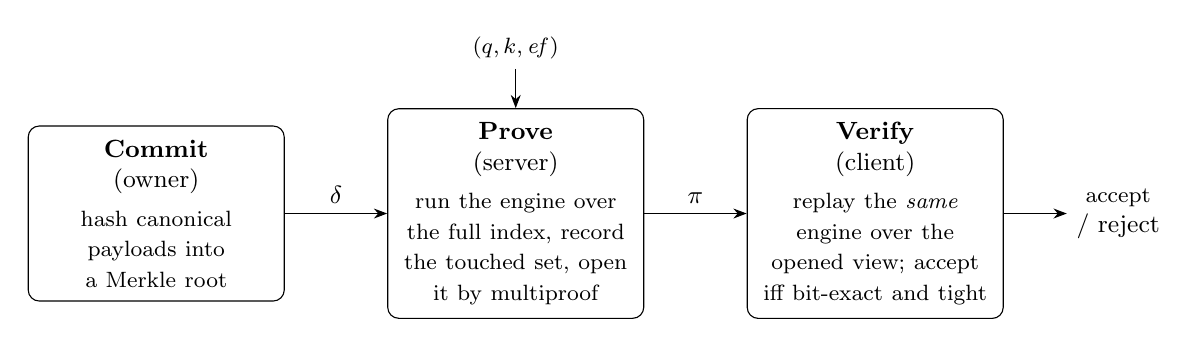
\begin{tikzpicture}[
  font=\small, >=Stealth,
  box/.style={draw, rounded corners, align=center, inner sep=5pt,
              minimum height=1.5cm, text width=2.9cm}
]
\node[box] (commit)
  {\textbf{Commit}\\(owner)\\[3pt]\footnotesize hash canonical
   payloads into a Merkle root};
\node[box, right=1.3cm of commit] (prove)
  {\textbf{Prove}\\(server)\\[3pt]\footnotesize run the engine over the
   full index, record the touched set, open it by multiproof};
\node[box, right=1.3cm of prove] (verify)
  {\textbf{Verify}\\(client)\\[3pt]\footnotesize replay the \emph{same}
   engine over the opened view; accept iff bit-exact and tight};
\draw[->] (commit) -- node[above]{$\delta$} (prove);
\draw[->] (prove) -- node[above]{$\pi$} (verify);
\node[above=0.5cm of prove] (q) {\footnotesize $(q,k,\mathit{ef})$};
\draw[->] (q) -- (prove);
\node[right=0.8cm of verify, align=center] (out)
  {\footnotesize accept\\/ reject};
\draw[->] (verify) -- (out);
\end{tikzpicture}
\caption{The \sys{} protocol. The owner commits the index to a digest
$\delta$; the server answers a query by running the deterministic
engine over the full index, recording the touched set, and opening
exactly those leaves as a proof $\pi$; the client, holding $\delta$,
replays the \emph{same} engine over the opened view and accepts only if
the replay reproduces the claimed result bit-for-bit and opens no more
than it uses. Because prover and verifier share one
\texttt{search\_with\_view} implementation, their agreement is
structural.}\label{fig:protocol}
\end{figure}

\section{Security Analysis}\label{sec:security}

\subsection{Objects and notation}

An index $I=(G,X)$ is committed together with its parameters
$P=(n,e^*,L,m,m_0,\mathit{dim},\mathit{metric})$. Here $G$ is a layered
graph over ids $[n]=\{0,\dots,n-1\}$: node $i$ exists on layers $0$
through $\mathrm{level}(i)$, its per-layer adjacency lists are canonical
(strictly ascending ids, no self-loops, degree at most $m_0$ at
layer~$0$ and $m$ above), and an edge at layer~$\ell$ points only to
nodes present at $\ell$. The map $X:[n]\to\mathbb{Z}_{8}^{\mathit{dim}}$
gives the quantized (int8) vectors, and $e^*$ is the entry point --- the
highest-level node, ties broken to the smallest id --- at level $L$.

Each node has a canonical payload
$\mathit{payload}_i=\mathrm{adjbytes}(i)\,\|\,\mathrm{vecbytes}(i)$, a
byte string with exactly one parse and, because the id is embedded in
$\mathrm{adjbytes}(i)$, distinct across nodes. The commitment is
$\delta=\mathsf{Commit}(I)=(\mathit{root},P)$, where $\mathit{root}$ is
the domain-separated, power-of-two-padded Merkle root over
$H_{\mathrm{leaf}}(\mathit{payload}_0),\dots,H_{\mathrm{leaf}}(\mathit{payload}_{n-1})$.

The reference computation is the deterministic search
$S(I,q,k,\mathit{ef})$: a greedy descent on layers $L$ down to $1$, a
best-first beam of width $\max(\mathit{ef},k,1)$ at layer~$0$, and
truncation to the $k$ closest. Every ordering is on the tuple
$(\mathit{dist},\mathit{id})$ and every distance is integer-exact, so
$S$ is a total function of its arguments --- no randomness, no platform
dependence.

\begin{definition}[Trace consistency]\label{def:tc}

Fix an index $I$ and its commitment $\delta=\mathsf{Commit}(I)$. A
verifier is \emph{trace-consistent} if accepting a transcript for a
query $(q,k,\mathit{ef})$ implies that the certified result equals
$S(I,q,k,\mathit{ef})$, the output of the canonical search on the
committed index. \sys{} achieves this computationally: the implication
fails only with the collision-finding advantage of
Theorem~\ref{thm:soundness}.

\end{definition}

\subsection{Building blocks}

\begin{lemma}[Merkle binding]\label{lem:binding}

Under collision resistance of the hash, no efficient adversary can
produce, for one $(\mathit{root},n,\mathit{position})$, two distinct
payloads whose openings both verify, except with negligible probability.
Domain separation (\texttt{0x00} leaf, \texttt{0x01} node, \texttt{0x02}
empty prefixes) rules out cross-domain second preimages, and the
verifier derives the expected proof depth from $n$, excluding shape
confusion. Padding positions $\ge n$ --- the power-of-two,
\texttt{0x02}-domain empty leaves --- cannot be opened as real nodes:
acceptance requires $\mathit{position}\in[0,n)$ through the
\texttt{decoded.id}${=}$\texttt{position} check, and an empty leaf's
hash lies in a domain disjoint from every $H_{\mathrm{leaf}}$.

\end{lemma}

\begin{lemma}[Locality]\label{lem:locality}

The execution of $S(I,q,k,\mathit{ef})$ reads a well-defined
\emph{touched set} $T(I,q,k,\mathit{ef})\subseteq[n]$ --- the ids whose
level, adjacency, or vector the engine accesses --- and the output of
$S$ depends only on $(q,k,\mathit{ef},P)$ and the restriction $I|_T$.
The engine reaches node data solely through an \texttt{IndexView}
interface, and a recording view materializes $T$.

\end{lemma}

\begin{lemma}[Replay coincidence]\label{lem:coincidence}

Let $V$ be any view over $[n]$ that agrees with $I$ wherever it answers:
for every id $u$ on which $V$ returns level, adjacency, or vector
without error, that data equals $I$'s. Running the fixed engine over $V$
with the committed $(e^*,L,P)$ and client $(q,k,\mathit{ef})$, exactly
one of the following holds. \emph{(i)} The engine requests data for some
$u\notin\mathrm{dom}(V)$ and aborts. \emph{(ii)} The engine never leaves
$\mathrm{dom}(V)$, and its step-by-step execution is identical to
$S(I,q,k,\mathit{ef})$: it touches the same set
$T'=T\subseteq\mathrm{dom}(V)$ and returns the same list.

\end{lemma}

\begin{proof}

The engine's control state after each step is a deterministic function
of $(q,k,\mathit{ef},P,e^*)$ and the sequence of view responses so far:
every branch tests only the parameters or $(\mathit{dist},\mathit{id})$
tuples whose distances are of already-read vectors and whose ids came
from already-read adjacency, with no ambient state, floating point, or
clock. Induct on execution steps. \emph{Base:} both runs start at $e^*$
with an empty visited set and empty heaps, hence in the same state.
\emph{Step:} assume identical state before the next access to $u$. If
$u\notin\mathrm{dom}(V)$, case~(i) fires. Otherwise $V$'s response for
$u$ equals $I$'s, so both runs receive identical data, take the
identical branch, and reach an identical successor state. The two traces
therefore coincide until, if ever, an out-of-domain access, giving~(i)
or~(ii).

\end{proof}

\subsection{The verifier}

$\mathsf{Verify}(\delta,q,k,\mathit{ef},\pi)$ proceeds in six stages:
(1) dimension and empty-index conventions; (2) batch Merkle verification
of all openings against $(\mathit{root},n)$; (3) strict payload decoding
with the position--identity check
\texttt{decoded.id}${=}$\texttt{position}; (4) replay of the \emph{same}
engine over the partial view built from the openings, aborting on any
access outside it; (5) bit-exact equality of the replayed list with
$\pi.\mathsf{result}$; and (6) a tightness check that the replay's
touched set equals the opened set.

The query parameters $(q,k,\mathit{ef})$ are client inputs to
$\mathsf{Verify}$, not fields of $\pi$: the server commits $\delta$
first and then answers whatever query the client issues, so it cannot
understate $\mathit{ef}$. Stage~(4) replays at beam
$\max(\mathit{ef},k,1)$ with the client's $\mathit{ef}$; a server that
searched at a smaller effective beam opened fewer leaves, so the
honest-$\mathit{ef}$ replay reaches a node it never opened and aborts.
The lazy-$\mathit{ef}$ guarantee is therefore not circular:
$\mathit{ef}$ is pinned by the client, echoed into the replay, and $T$
is taken at that $\mathit{ef}$.

\subsection{Soundness}

The bound below holds under four standing assumptions. \textbf{(A1)} the
hash (blake3) is collision resistant. \textbf{(A2)} the verifier replays
the \emph{same} engine that defines $S$ --- a single
\texttt{search\_with\_view} generic over \texttt{IndexView} --- so
prover and verifier agree by construction rather than through a
duplicated implementation. \textbf{(A3)} arithmetic is integer-exact
with a total $(\mathit{dist},\mathit{id})$ order and hash-derived
levels, making $S$ platform-independent and replay bit-exact.
\textbf{(A4)} the batched multiproof verifier accepts a set of openings
iff each constituent per-leaf opening would. Only (A1) enters the bound;
(A2)--(A4) license the steps of the proof.

\begin{theorem}[Soundness]\label{thm:soundness}

Let $\delta=\mathsf{Commit}(I)$. For every PPT adversary $\mathcal{A}$
outputting $(q,k,\mathit{ef},\pi)$,
\[
\Pr\!\left[\mathsf{Verify}(\delta,q,k,\mathit{ef},\pi)=1 \;\wedge\; \pi.\mathsf{result}\neq S(I,q,k,\mathit{ef})\right] \;\le\; \mathsf{Adv}^{\mathrm{CR}}_{\mathrm{blake3}}(\mathcal{B}),
\]
for an explicit reduction $\mathcal{B}$ that extracts a blake3 collision
from any accepting, deviating transcript.

\end{theorem}

\begin{proof}

Suppose $\mathsf{Verify}$ accepts. By Lemma~\ref{lem:binding}, every
opened payload equals $I$'s payload at its position: a mismatch would
yield two verifying openings for one position, from which $\mathcal{B}$
(below) extracts a collision. Stage~(3)'s identity check forbids
transplanting node $j$'s content to position $i$, so the opened view $V$
is a restriction of $I$ --- exactly the hypothesis of
Lemma~\ref{lem:coincidence}. Since Stage~(4) ran to completion, case~(i)
of that lemma (a \texttt{MissingNode} abort) is excluded, so case~(ii)
holds: the replay touches exactly $T(I,q,k,\mathit{ef})$ and returns
$S(I,q,k,\mathit{ef})$. Stage~(5) then forces
$\pi.\mathsf{result}=S(I,q,k,\mathit{ef})$, contradicting the assumed
deviation.

\end{proof}

\noindent\textbf{The reduction $\mathcal{B}$.} $\mathcal{B}$ holds $I$
(which fixes $\delta$) and the accepting, deviating transcript. At the
deviating position $i$ it has two payloads --- the transcript's
$\mathit{payload}^{\mathcal{A}}$ and $I$'s true $\mathit{payload}^{I}$
--- that differ yet both verify against $\mathit{root}$. It recomputes
$i$'s honest authentication path from $I$ and walks it against the
transcript's path from the leaf upward. If
$H_{\mathrm{leaf}}(\mathit{payload}^{\mathcal{A}})=H_{\mathrm{leaf}}(\mathit{payload}^{I})$
while the payloads differ, that leaf pair is already a collision;
otherwise the leaf hashes differ and $\mathcal{B}$ ascends to the first
internal level whose two nodes carry equal hashes but distinct child
pairs, a collision of $H_{\mathrm{node}}$. Domain separation keeps the
colliding inputs in one domain. Because $\mathcal{B}$ locates the
divergence deterministically against $I$ rather than guessing, no factor
of $|T|$ or $n$ enters and the bound carries no slack.

\begin{proposition}[Completeness]\label{prop:complete}

The honest prover runs the same engine over the full index and opens
exactly the recorded touched set; its proofs therefore always verify. In
debug builds the prover self-checks this.

\end{proposition}

\begin{proposition}[Tightness]\label{prop:tight}

If $\mathsf{Verify}$ accepts, the opened set equals
$T(I,q,k,\mathit{ef})$: Lemma~\ref{lem:coincidence}(ii) gives $T'=T$,
Stage~(4) rules out omissions (\texttt{MissingNode}), and Stage~(6)
rules out padding (\texttt{UnusedOpenings}). Hence
$|\mathit{VO}|=\Theta(|T|\cdot(\mathit{payload}+\text{amortized path}))$
--- the proof is precisely the search's data footprint, and reported
proof sizes are not gameable in either direction.

\end{proposition}

\subsection{Scope}

We close by delimiting what the guarantee does and does not claim.

\begin{itemize}
\item \emph{Execution, not optimum.} Verifying the true top-$k$ of an
  approximate index is either meaningless or as costly as exact search;
  trace consistency instead binds the answer to the canonical execution
  on the committed index, catching result tampering, lazy $\mathit{ef}$,
  entry-point games, and stale copies at per-query cost.
\item \emph{Quality lives in the commitment.} A server may commit a poor
  index but cannot misrepresent what that index returns; clients
  calibrate expectations from the committed parameters and published
  recall curves.
\item \emph{Adaptivity adds nothing.} $\delta$ is fixed before queries
  and each verification is stateless and per-query, so the bound
  survives any adaptive strategy by a union bound over queries.
\item \emph{Which resource is sublinear.} Succinctness is in $n$:
  $|\mathit{VO}|=\Theta(|T|\cdot(\mathit{payload}+\text{amortized
  path}))$ with $|T|\ll n$, tracking the search's footprint rather than
  the index. Dependence on $d$ is linear at Tier-1 (each opened payload
  carries a raw $d$-vector) and is the target of the Tier-2 aggregated
  inner-product argument (\S\ref{sec:discussion}); verifier time is
  $O(|T|\cdot\deg\cdot\mathit{dim}+|\mathit{VO}|\cdot\mathit{hash})$ and
  its working memory is $O(n)$ for an $n$-bit visited bitmap. We
  headline $|\mathit{VO}|$ and do not claim sublinear verifier space.
\end{itemize}

\section{Implementation}\label{sec:impl}

\sys{} is a Rust workspace of about $3{,}000$ lines across four crates:
\texttt{ta-core} (the deterministic engine, the graph, and the view
interface, $1{,}303$ lines), \texttt{ta-commit} (canonical payloads, the
domain-separated Merkle tree, and multiproofs, $671$ lines),
\texttt{ta-proof} (the prover, the six-stage verifier, and the
adversarial test suite, $477$ lines), and \texttt{ta-bench} (the
measurement harness, $581$ lines). The only external dependency is the
\texttt{blake3} hash; there is no GPU code and no floating point on the
query path. The suite has $42$ tests, and because every proof produced
during a benchmark sweep is verified, the harness doubles as a large
randomized end-to-end test. Two guardrails protect the properties the
paper depends on: a golden-digest test asserts that a fixed index and
query hash to the same bytes on x86-64 Linux and aarch64 macOS --- a
determinism regression stops the build --- and in debug builds the
prover verifies its own proof before returning it.

\section{Evaluation}\label{sec:eval}

\subsection{Setup}

All timings are single-threaded on one core of an Apple M1 Pro
(MacBook Pro 14-inch, 2021) with 16\,GB of unified memory. Each operation ---
plaintext search, prove, verify --- is run three times per query and the
minimum wall time is kept as the best estimator of intrinsic cost under
scheduler noise; tables report the median and, where noted, the p95
across the query set. Proof-size metrics (opened leaves and wire bytes)
are exact and, like the commitments, reproduce byte-for-byte on any
machine, so only latencies are hardware-dependent.

Two data regimes are used. The synthetic \emph{clustered} generator
plants points in roughly $32$-point clusters whose centroids occupy a
fixed ${\sim}16$-dimensional global subspace, with each cluster adding
noise in its own ${\sim}16$-dimensional subspace; intrinsic
dimensionality is therefore held near $32$ while the ambient dimension
$d$ varies, mirroring real embedding models and letting the $d$ sweep
isolate the payload term of the proof with the opened-leaf count roughly
flat. The design is deliberate: uniform random data concentrates
distances and collapses recall, full-dimensional cluster noise reduces
to the same high-dimensional uniform subproblem, clusters larger than
the construction beam degenerate layer~$0$ into disconnected islands,
and uniform random centroids leave no gradient for coarse navigation ---
each generator knob fixes one of these failure modes we observed
empirically. The real regime is SIFT1M: its descriptors are integers in
$[0,255]$, and the affine shift $q=x-128$ embeds them into int8
losslessly (squared Euclidean distance is translation-invariant), so
recall is measured against the official float ground truth with no
quantization confound.

\subsection{End-to-end cost on SIFT1M}

Table~\ref{tab:sift} and Figure~\ref{fig:sift} report the end-to-end
cost on a one-million-vector index. At $\mathit{ef}=64$ the engine
reaches recall@$10=0.956$ while opening $1{,}217$ of the million leaves;
the resulting proof is $607$\,KiB, produced in $325\,\mu$s ---
$8.4\times$ a plaintext search --- and verified in $2.7$\,ms. Sweeping
$\mathit{ef}$ traces a smooth accuracy--cost frontier: recall climbs
from $0.771$ to $0.996$ as the proof grows from $250$ to $1{,}689$\,KiB
and verification from $1.1$ to $7.3$\,ms, with prover overhead holding
near $8\times$ throughout. The one-off costs --- a $0.59$\,s commitment
and a $307$\,s index build --- are amortized over the lifetime of the
index and irrelevant to per-query verification.

\begin{table}[t]\centering
\caption{SIFT1M ($n{=}10^6$, $d{=}128$, $m{=}16$,
$\mathit{ef}_c{=}200$): recall vs.\ official ground truth and
verification costs.}\label{tab:sift}
% Auto-generated by bench/plot_results.py -- do not edit by hand.
\begin{tabular}{rrrrrrr}
\toprule
$ef$ & recall@$k$ & opened & VO (KiB) & search ($\mu$s) & prove ($\mu$s) & verify (ms) \\
\midrule
16 & 0.771 & 449 & 250 & 16 & 127 (8.1$\times$) & 1.1 \\
32 & 0.884 & 717 & 379 & 23 & 195 (8.4$\times$) & 1.7 \\
64 & 0.956 & 1217 & 607 & 39 & 325 (8.4$\times$) & 2.7 \\
128 & 0.986 & 2153 & 1004 & 75 & 564 (7.5$\times$) & 4.4 \\
256 & 0.996 & 3853 & 1689 & 144 & 1212 (8.4$\times$) & 7.3 \\
\bottomrule
\end{tabular}

\end{table}

\begin{figure}[t]\centering
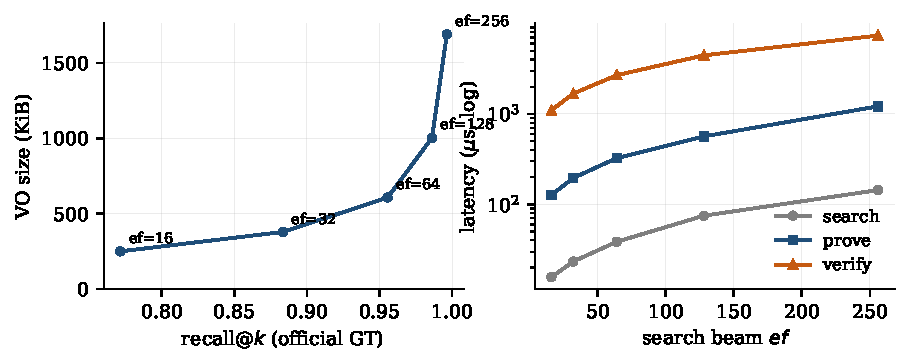
\includegraphics[width=\linewidth]{fig4_sift1m.pdf}
\caption{SIFT1M: VO size along the recall Pareto frontier (left) and
search/prove/verify latencies (right).}\label{fig:sift}
\end{figure}

\subsection{Controlled sweeps}

The ambient-dimension sweep (Figure~\ref{fig:d}, Table~\ref{tab:d})
isolates how the proof scales with $d$ at fixed intrinsic dimension. As
$d$ grows from $64$ to $768$ the number of opened leaves does not rise
--- it drifts down from $938$ to $554$ --- yet the proof grows from
$290$ to $556$\,KiB, because each opened payload carries a raw $d$-byte
vector: the growth is entirely in the payload term, exactly the Tier-1
behavior the succinct tier is meant to remove (\S\ref{sec:discussion}).
Prover overhead relative to plaintext search falls from $11.9\times$ to
$3.5\times$ over the same range, since hashing the touched set is nearly
$d$-independent while the plaintext distance work it is measured against
grows with $d$.

\begin{figure}[t]\centering
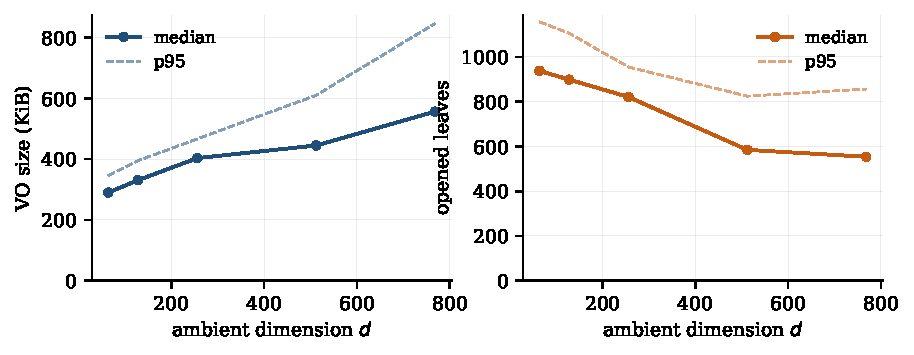
\includegraphics[width=\linewidth]{fig1_vo_vs_d.pdf}
\caption{Fixed intrinsic dimension, varying ambient $d$: VO grows with
the payload term while opened leaves do not.}\label{fig:d}
\end{figure}

\begin{table}[t]\centering
\caption{Ambient-dimension sweep ($n{=}50$k, $\mathit{ef}{=}64$).}
\label{tab:d}
% Auto-generated by bench/plot_results.py -- do not edit by hand.
\begin{tabular}{rrrrrrrr}
\toprule
$d$ & recall@$k$ & opened & VO (KiB) & B/leaf & prove ($\mu$s) & verify ($\mu$s) & overhead \\
\midrule
64 & 0.910 & 938 & 290 & 317 & 223 & 1482 & 11.9$\times$ \\
128 & 0.725 & 899 & 331 & 377 & 202 & 1440 & 8.3$\times$ \\
256 & 0.950 & 821 & 404 & 503 & 204 & 1452 & 5.9$\times$ \\
512 & 0.835 & 585 & 445 & 779 & 165 & 1268 & 4.3$\times$ \\
768 & 0.950 & 554 & 556 & 1029 & 170 & 1378 & 3.5$\times$ \\
\bottomrule
\end{tabular}

\end{table}

The effort sweep (Figure~\ref{fig:ef}) confirms that $\mathit{ef}$ is
the single knob trading verification cost for accuracy: recall and proof
size rise together as the beam widens, so a client selects its point on
the frontier by the recall it needs and pays proportionally in proof
bytes and verification time.

\begin{figure}[t]\centering
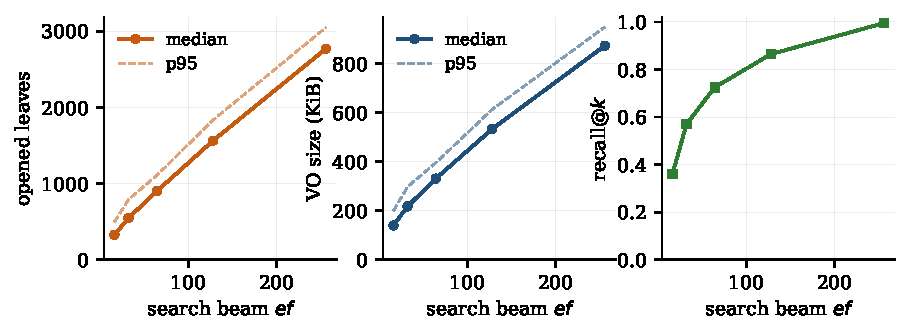
\includegraphics[width=\linewidth]{fig2_vo_vs_ef.pdf}
\caption{Effort sweep: recall and VO both rise with $\mathit{ef}$, the
knob that trades verification cost for accuracy.}\label{fig:ef}
\end{figure}

The index-size sweep (Figure~\ref{fig:n}, log-scaled in $n$) shows the
opened-leaf count --- and thus the proof --- growing far more slowly
than the index, the property that keeps verification succinct as the
corpus scales. One caveat is specific to the synthetic generator: recall
dips around $n=10^5$ because the fixed $16$-dimensional centroid
subspace saturates at roughly $n/32$ clusters; this is an artifact of
the data model, not the index, and the real SIFT1M results at $n=10^6$
are unaffected.

\begin{figure}[t]\centering
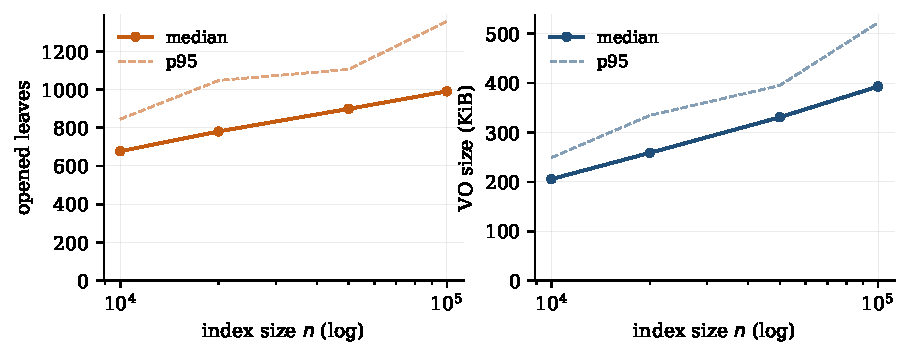
\includegraphics[width=\linewidth]{fig3_vo_vs_n.pdf}
\caption{Index-size sweep (log $x$): opened leaves grow far slower than
$n$, so the proof stays succinct as the index scales.}\label{fig:n}
\end{figure}

\subsection{Attack detection}

Finally, the adversarial suite in \texttt{ta-proof} instantiates each
server behavior from the threat model of \S\ref{sec:model} and confirms
that it is rejected --- not by a catch-all check, but by the specific
stage the design assigns to it (Table~\ref{tab:attacks}). Tampering with
committed data or answering from a different index fails Merkle
verification; identity forgery and malformed payloads fail strict
decoding; a lazy or truncated search is caught when the honest-parameter
replay reaches an unopened node; a doctored result fails the bit-exact
comparison; and a padded proof fails the tightness check. The mapping is
exhaustive over the capabilities enumerated in \S\ref{sec:model}.

\begin{table}[t]\centering\footnotesize
\caption{Every adversarial behavior from \S\ref{sec:model} is rejected
by a specific verification stage, as exercised by the \texttt{ta-proof}
attack suite.}\label{tab:attacks}
\begin{tabular}{@{}lcl@{}}
\toprule
Attack & Stage & Rejecting check \\
\midrule
Non-empty result on an empty index & (1) & \texttt{EmptyIndexNonEmptyResult} \\
Modified vector or edge            & (2) & \texttt{BadOpening} \\
Proof against a different index     & (2) & \texttt{BadOpening} \\
A required opening dropped          & (2) & \texttt{BadOpening} \\
Node $j$ served at position $i$     & (3) & \texttt{IdMismatch} \\
Non-canonical / malformed payload   & (3) & \texttt{MalformedPayload} \\
Lazy or smaller-$\mathit{ef}$ search & (4) & \texttt{MissingNode} \\
Reordered or substituted top-$k$    & (5) & \texttt{ResultMismatch} \\
Proof padded with unused leaves     & (6) & \texttt{UnusedOpenings} \\
\bottomrule
\end{tabular}
\end{table}

\section{Discussion and Future Work}\label{sec:discussion}

The one place \sys{}'s proof is not succinct is its dependence on the
ambient dimension: every opened leaf carries a raw $d$-byte vector, so
the verification object grows linearly in $d$ (\S\ref{sec:eval},
Figure~\ref{fig:d}). The design anticipates a second tier that removes
this. Because a leaf payload is
$\mathrm{adjbytes}(i)\,\|\,\mathrm{vecbytes}(i)$ and the Merkle
machinery hashes payloads opaquely, the raw vector can be replaced by a
constant-size ($32$-byte) Pedersen commitment to that vector without
touching the commitment structure or the traversal logic at all --- the
graph, the domain separation, and the six-stage verifier are unchanged.
The distances the replay recomputes are then discharged not by
re-reading vectors but by a single aggregated inner-product argument
\cite{bunz2018bulletproofs} over all touched nodes, whose size is
logarithmic in the total coordinate count rather than linear in $d$ per
node. This turns the $d$-linear payload term of Table~\ref{tab:d} into a
sublinear one while preserving trace consistency, which is why we report
the Tier-1 numbers as a floor rather than a limit.

\sys{} today verifies against a single committed snapshot; the freshness
of that snapshot across re-commitments is out of scope
(\S\ref{sec:model}). The natural extension is a journaled commitment:
each update publishes a new root together with a signed link to its
predecessor, forming a hash chain of epochs that a client can audit for
monotonic progress and against which a server cannot silently roll back.
Combined with the sharding-style incremental updates that graph-based
authenticated indexes already support, this would carry trace
consistency from a static index to a mutable one without changing the
per-query proof.

Two further directions follow naturally. First, real retrieval
increasingly couples nearest-neighbor search with metadata predicates;
extending trace consistency to \emph{filtered} search --- proving that
the returned results are exactly those the canonical traversal visits
subject to a committed predicate --- would cover a large class of
production queries, and the deterministic-execution framing transfers
directly. Second, the integer-exact distance kernels are associative by
construction (\S\ref{sec:design}), so a SIMD or GPU implementation may
reorder accumulation freely; this promises a large constant-factor
speedup in both proving and verification with no effect on the committed
bytes, since determinism is a property of the arithmetic, not the
schedule.

Two limitations bound the present results. The synthetic generator's
recall degrades beyond $n\approx10^5$ as its fixed low-dimensional
centroid subspace saturates (\S\ref{sec:eval}); this is a property of
the benchmark, not the index, and the real SIFT1M results are
unaffected, but a generator whose global subspace scales with $\log n$
would make the synthetic $n$ sweep faithful at larger scales. And by
design \sys{} reveals the query's access pattern through the set of
opened nodes --- the cost of an always-on, single-server,
non-interactive proof; applications that must hide the access pattern
need the heavier zero-knowledge machinery discussed in
\S\ref{sec:related}, at a per-query cost incompatible with the always-on
setting \sys{} targets.

\section{Conclusion}\label{sec:conclusion}

\sys{} shows that integrity for graph-based approximate nearest-neighbor
search can be made always-on and cheap by verifying the \emph{execution}
rather than the optimum: a returned result is accepted only if it is
bit-for-bit the output of a canonical, deterministic search over a
Merkle-committed index, a property we prove sound by reduction to a hash
collision. On a million-vector SIFT1M index this costs a $607$\,KiB
proof and $2.7$\,ms of client verification per query at $0.956$ recall,
driven by a reproducible, integer-exact engine whose commitments match
to the byte across architectures. The complete system is open source,
and its layered commitment leaves a clear path to proofs that are
succinct in the ambient dimension as well.

\bibliographystyle{plain}
\bibliography{refs}

\end{document}
